\documentclass[10pt,a4paper,onecolumn]{article}
% \usepackage[utf8]{inputenc}
\usepackage{marginnote}
\usepackage{graphicx}
\usepackage{xcolor}
\usepackage{authblk,etoolbox}
\usepackage{titlesec}
\usepackage{calc}
\usepackage{hyperref}
\hypersetup{breaklinks=true,
            bookmarks=true,
            pdfauthor=
{
      Vahid Rostami,
      Junji Ito,
      Michael Denker,
      Sonja Grün,
  },
            pdftitle=
{
[Re] Spike Synchronization and Rate Modulation Differentially Involved in
Motor Cortical Function
},
            colorlinks=true,
            citecolor=blue,
            urlcolor=blue,
            linkcolor=blue,
            pdfborder={0 0 0}}
\urlstyle{same}
\usepackage{tcolorbox}
\usepackage{ragged2e}
\usepackage{fontspec}
\usepackage{fontawesome}
\usepackage{caption}
\usepackage{listings}
\lstnewenvironment{code}{\lstset{language=Haskell,basicstyle=\small\ttfamily}}{}



%\usepackage{fancyvrb}
%\VerbatimFootnotes
%\usepackage{graphicx}
%\usepackage{mdframed}
%\newmdenv[backgroundcolor=lightgray]{Shaded}


\usepackage{longtable,booktabs}

\usepackage[
  backend=biber,
%  style=alphabetic,
%  citestyle=numeric
]{biblatex}
\bibliography{VRostami_JIto_MDenker_SGruen_2016.bib}



% --- Macros ------------------------------------------------------------------
\renewcommand*{\bibfont}{\small \sffamily}

\definecolor{red}{HTML}{CF232B}
\newcommand{\ReScience}{Re{\bfseries \textcolor{red}{Science}}}

\newtcolorbox{rebox}
   {colback=blue!5!white, colframe=blue!40!white,
     boxrule=0.5pt, arc=2pt, fonttitle=\sffamily\scshape\bfseries,
     left=6pt, right=20pt, top=6pt, bottom=6pt}

\newtcolorbox{repobox}
   {colback=red, colframe=red!75!black,
     boxrule=0.5pt, arc=2pt, left=6pt, right=6pt, top=3pt, bottom=3pt}

% fix for pandoc 1.14     
\newcommand{\tightlist}{%
  \setlength{\itemsep}{1pt}\setlength{\parskip}{0pt}\setlength{\parsep}{0pt}}

% --- Style -------------------------------------------------------------------
\renewcommand*{\bibfont}{\small \sffamily}
\renewcommand{\captionfont}{\small\sffamily}
\renewcommand{\captionlabelfont}{\bfseries}

\makeatletter
\renewcommand\@biblabel[1]{{\bf #1.}}
\makeatother

% --- Page layout -------------------------------------------------------------
\usepackage[top=3.5cm, bottom=3cm, right=1.5cm, left=1.5cm,
            headheight=2.2cm, reversemp, includemp, marginparwidth=4.5cm]{geometry}

% --- Section/SubSection/SubSubSection ----------------------------------------
\titleformat{\section}
  {\normalfont\sffamily\Large\bfseries}
  {}{0pt}{}
\titleformat{\subsection}
  {\normalfont\sffamily\large\bfseries}
  {}{0pt}{}
\titleformat{\subsubsection}
  {\normalfont\sffamily\bfseries}
  {}{0pt}{}
\titleformat*{\paragraph}
  {\sffamily\normalsize}


% --- Header / Footer ---------------------------------------------------------
\usepackage{fancyhdr}
\pagestyle{fancy}
%\renewcommand{\headrulewidth}{0.50pt}
\renewcommand{\headrulewidth}{0pt}
\fancyhead[L]{\hspace{-1cm}\includegraphics[width=4.0cm]{rescience-logo.pdf}}
\fancyhead[C]{}
\fancyhead[R]{} 
\renewcommand{\footrulewidth}{0.25pt}

\fancyfoot[L]{\hypersetup{urlcolor=red}
              \sffamily \ReScience~$\vert$
              \href{http://rescience.github.io}{rescience.github.io}
              \hypersetup{urlcolor=blue}}
\fancyfoot[C]{\sffamily \thepage}
\fancyfoot[R]{\sffamily Nov 2016 $\vert$
                        Volume \textbf{1} $\vert$
                        Issue \textbf{1}}
\pagestyle{fancy}
\makeatletter
\let\ps@plain\ps@fancy
\fancyheadoffset[L]{4.5cm}
\fancyfootoffset[L]{4.5cm}

% --- Title / Authors ---------------------------------------------------------
% patch \maketitle so that it doesn't center
\patchcmd{\@maketitle}{center}{flushleft}{}{}
\patchcmd{\@maketitle}{center}{flushleft}{}{}
% patch \maketitle so that the font size for the title is normal
\patchcmd{\@maketitle}{\LARGE}{\LARGE\sffamily}{}{}
% patch the patch by authblk so that the author block is flush left
\def\maketitle{{%
  \renewenvironment{tabular}[2][]
    {\begin{flushleft}}
    {\end{flushleft}}
  \AB@maketitle}}
\makeatletter
\renewcommand\AB@affilsepx{ \protect\Affilfont}
%\renewcommand\AB@affilnote[1]{{\bfseries #1}\hspace{2pt}}
\renewcommand\AB@affilnote[1]{{\bfseries #1}\hspace{3pt}}
\makeatother
\renewcommand\Authfont{\sffamily\bfseries}
\renewcommand\Affilfont{\sffamily\small\mdseries}
\setlength{\affilsep}{1em}

\LetLtxMacro{\OldIncludegraphics}{\includegraphics}
\renewcommand{\includegraphics}[2][]{\OldIncludegraphics[width=12cm, #1]{#2}}


% --- Document ----------------------------------------------------------------
\title{[Re] Spike Synchronization and Rate Modulation Differentially Involved in
Motor Cortical Function}

    \usepackage{authblk}
                        \author[1]{Vahid Rostami}
                    \author[1]{Junji Ito}
                    \author[1]{Michael Denker}
                    \author[1,2]{Sonja Grün}
                            \affil[1]{Inst. of Neuroscience \& Medicine (INM-6) and Inst. for Advanced
Simulation (IAS-6), JARA Brain Institute I, Jülich Research Center,
Jülich, Germany}
                    \affil[2]{Theoretical Systems Neurobiology, RWTH Aachen University, Aachen,
Germany}
            
\date{\vspace{-5mm}
      \sffamily \small \href{mailto:v.rostami@fz-juelich.de}{v.rostami@fz-juelich.de}}


\setlength\LTleft{0pt}
\setlength\LTright{0pt}


\begin{document}
\maketitle

\marginpar{
  %\hrule
  \sffamily\small
  %\vspace{2mm}
  {\bfseries Editor}\\
  Name Surname\\

  {\bfseries Reviewers}\\
        Name Surname\\
        Name Surname\\
  
  {\bfseries Received}  Nov, 1, 2016\\
  {\bfseries Accepted}  Nov, 1, 2016\\
  {\bfseries Published} Nov, 1, 2016\\

  {\bfseries Licence}   \href{http://creativecommons.org/licenses/by/4.0/}{CC-BY}

  \begin{flushleft}
  {\bfseries Competing Interests:}\\
  The authors have declared that no competing interests exist.
  \end{flushleft}

  \hrule
  \vspace{3mm}

  \hypersetup{urlcolor=white}
  
    \vspace{-1mm}
  \begin{repobox}
    \bfseries\normalsize
      \href{http://github.com/rescience/rescience-submission/article}{\faGithubAlt~Article repository}
  \end{repobox}
      \vspace{-1mm}
  \begin{repobox}
    \bfseries\normalsize
      \href{http://github.com/rescience/rescience-submission/code}{\faGithubAlt~Code repository}
  \end{repobox}
        \hypersetup{urlcolor=blue}
}

\begin{rebox}
\sffamily {\bfseries A reference implementation of}
\small
\begin{flushleft}
\begin{itemize}
    \item[→] Spike synchronization and rate modulation differentially involved in
motor cortical function. Alexa Riehle, Sonja Grün, Markus Diesmann, and
Ad Aertsen (1997) Science 278:1950-1953. DOI:10.1126/science.278.5345.19
50
  \end{itemize}\par
\end{flushleft}
\end{rebox}


\section{Introduction}\label{introduction}

Understanding how information is processed by networks of neurons in the
brain is a major goal in neuroscience. There has been a long-standing
debate in the community on the contribution of the firing activity of
individual neurons or populations of neurons to information processing:
one perspective is that the firing rate of the neurons, i.e.~the number
of spikes per time unit, represents information or is relevant for the
processing. Another perspective is that neurons communicate through
precisely timed coordination of spiking, a view that results from the
insight that a neuron fires most efficiently if it receives synchronous
spike input, i.e., in the range of a few milliseconds
\autocite{Abeles82}.

To test whether temporal coordination of spiking activity is indeed
relevant for neuronal information processing, advanced data analysis
methods are required that perform correlation analysis between
simultaneously recorded single unit spike trains. The Unitary Events
(UE) analysis method \autocites{GruenPhD}{Gruen99}{Gruen02a}{Gruen02b}
is able to extract significant spike synchrony between neuronal
activities that is beyond what is expected by chance (given the rates)
and to follow the dynamics of this coordination. The tricky issue with
such analyses is that one has to take into account that experimental
spike data are typically non-stationary in the sense that the firing
rates are not stationary in time and not homogeneous across trials, and
that the statistics of the individual spike trains deviate from those of
a Poisson process \autocites{Gruen09}{GruenRotter10_Chap10}. If such
features are ignored there is a considerable danger of occurrence of
false positives and thus wrong interpretation of the data. In
particular, changes in the firing rates are the most prominent
generators of false positives if ignored. The original UE method
considers this aspect by performing the analysis in a sliding time
window fashion. In later versions of the analysis method other features
were corrected for by considering the respective features in the
null-hypothesis of the tests
\autocites{Gruen03b}{Maldonado08}{Louis10}{Pipa2013}, either by using
extended analytical descriptions of the null-hypotheses or by use of
surrogate methods \autocites{Gruen09}{GruenRotter10_Chap10}{Louis10}.

The UE method had been applied to experimental parallel spike data from,
e.g., the motor cortex of awake behaving non-human primates
\autocites{Riehle97}{Gruen99}{Grammont99}{Riehle2000}{Gruen03b}{Kilavik09}{Denker10}{Denker11}
and to data from visual cortices \autocites{Maldonado08}{Ito11}.
Generally it was found that UEs, i.e., synchronous spike events across
neurons that are in excess of the expectation, occur in relation to
behavior, e.g., when the animal expects a signal to occur, however the
signal does not occur \autocite{Riehle97}. This finding, in particular,
demonstrates the core feature of the method: by performing a time
resolved analysis, the method accounts for changes in the firing rates
and captures modulations of significant spike synchrony in time. It was
also shown that the time of occurrence of UEs may change to a new
requested timing in the behavior during a learning process
\autocite{Kilavik09}.

Several of these studies based on the UE method, in particular
\autocite{Riehle97}, have been widely cited and the method has been
recognized as one of the standard tools to analyze temporal coordination
of neuronal spiking activities \autocites{Brown04_456}{Nakahara02}. The
analysis method has been and is taught in international data analysis
courses. However, a publicly available and open source implementation of
the UE method had not been available. Only very recently, one of the
authors of this study (VR) reimplemented the UE analysis as part of the
Electrophysiology Analysis Toolbox\footnote{\url{http://neuralensemble.org/elephant/}}
(Elephant), a Python library that provides implementations for the
analysis of electrophysiological data. This reimplementation of the
method was particularly required for, in addition to the general
motivation for a reimplementation to confirm the results not depending
on small implementation details or mistakes, the following two specific
reasons.

First, the custom data object model used to represent the primary data
and metadata in the original analysis code was not documented.
Therefore, any data represented in a specific file format had to be
converted by implementing a custom data loading routine for this data
model. Our new implementation of the UE method is part of the Elephant
and Neo\footnote{\url{http://neuralensemble.org/neo/}} libraries and is
based on the internal data object model provided by the Neo library
\autocite{Garcia14}, a package for representing electrophysiology data
in Python. Neo provides support for reading a wide range of
neurophysiology proprietary file formats, and supports writing to a
subset of these formats, including non-proprietary formats such as HDF5.

Second, the implementation of the UE method in the original publication
has experienced several updates after its publication in order to
include improvements and extensions of the method to accommodate more
features of experimental data. Since no version control was employed in
this development process, the original code used in Riehle et al.
\autocite{Riehle97} was lost at some point. Considering that no
systematic testing was performed each time the code base of the Unitary
Event analysis was updated after the original publication to check
whether the code gives the same results as before, it was not clear
whether the latest version could exactly reproduce the results of
\autocite{Riehle97}.

In this paper we illustrate the successful reproduction of the results
shown in \autocite{Riehle97} using our new Python implementation of the
UE method. In particular, we reproduce Figure 2 and Figure 4A of the
original paper, which represent the central results of the original
study. The remainder of the original paper consisted of more example
analyses of individual data sets and a meta statistics across many data
sets, all of which were based on the same analysis method and thus do
not provide additional insight when reproduced. In the original
publication the authors used two different UE implementations: one
implemented by one of the coauthors of the present study (SG) in
IDL\footnote{\url{http://www.harrisgeospatial.com/ProductsandSolutions/GeospatialProducts/IDL.aspx}},
and the other in Matlab (Mathworks, Nattick, MA) implemented later by
Markus Diesmann (MD) and SG. The IDL implementation is not available
anymore. At a later point we were provided with a Matlab implementation
of the extended UE method, however it does not preserve the original
implementation used in \autocite{Riehle97} and was not considered in
this study.

For the reproduction of the original results we contacted and
communicated with Alexa Riehle (AR), CNRS-AMU, Marseille, and MD,
Research Centre Jülich. AR is the first author of the original
publication and performed the experiments and data analysis. MD is the
third author of the original publication and contributed with the Matlab
implementation and quality checks of the software implementations. The
reproduction of the results of \autocite{Riehle97} would not have been
possible without contacting these authors, since the information in the
original publication is not sufficient for reproducing the results. AR
provided us with the original data and information, including an old
written report by MD, which was crucial to reproduce Figure 4A.

\section{Methods}\label{methods}

For reproducing the results of \autocite{Riehle97} we use our
reimplementation of the UE analysis method in Python which is made
available in the \texttt{unitary\_event\_analysis} module of the
Elephant library (accepted pull-request: \autocite{Pullrequest_UE}). The
method is accompanied by unit tests for individual functions (test
coverage: \(88.54\%\)) and documented as part of the library
documentation. The structure and algorithm of our UE implementation is
explained in the pseudo-code shown below.

In the following, we will explain the algorithm in detail. The primary
data entering the UE method is a set of parallel, i.e., simultaneously
recorded, spike trains, recorded in one or multiple trials. In Elephant,
an individual spike train of a particular neuron in a particular trial
data is represented as a \texttt{Spiketrain} object in the data object
model provided by the Neo library, which stores the time points of spike
occurrences along with additional information describing the spike
train, such as the start and end times. The UE method consumes a nested
list of \texttt{Spiketrain} objects relating to the spike trains of
individual neurons in the individual trials. In order to perform the
necessary calculations, the spike data must be converted to an
alternative time-binned representation (line 1 in the pseudo code) where
the parallel spike trains are stored as binary sequences of ones
(marking time bins containing at least 1 spike) and zeros (bins with no
spike). The bin size is a parameter provided as input (parameter
\emph{\texttt{bin\_size}} in the pseudo code) to the analysis, and
defines the temporal precision in detecting spike synchrony. A spike
pattern, which is a representation of spike synchrony in the analysis,
is defined as a specific vector of zeros and ones in one time bin of a
given trial across all neurons. Since the aim of the UE method is to
detect significant spike synchrony, the total number of spike patterns
of concern is given by \(2^{N}-N-1\), where \(N\) is the number of
neurons, the first term is the number of all possible spike patterns,
the second term is the number of spike patterns composed of only one
spike, and the third term is the number of the pattern without a spike.
In order to limit the analysis to a set of patterns of interest, the
input parameter \emph{\texttt{pattern\_hash\_values}} specifies the
patterns to consider in the analysis in the form of a hash value which
uniquely represents each spike pattern (line 2 in the pseudo code). The
hash value is obtained by interpreting the binary spike pattern as a
binary number, where the \(n\)-th neuron is represented by bit \(n-1\).

The UE analysis is performed in a sliding time window fashion, i.e.~the
data in each window are analyzed separately. This approach is chosen to
account for potential changes of the firing rates in time and to follow
the dynamics of the correlation. Here, a sliding time window is defined
based on trial time, meaning that a certain window position includes the
activity of all neurons in all trials in a certain time interval of the
trial. In the algorithm, at each position of the window, the data
contained in the window are extracted in order to compute the
significance of the specified patterns (line 3 in the pseudo code). For
doing that the UE analysis requires the empirical number of occurrences
of each pattern as well as its expected number given the firing rates.
While the empirical number is directly extracted from the data (line 5
in the pseudo code), the method to compute the expected number can be
chosen using the input parameter \emph{\texttt{method}} depending on the
assumptions regarding the data (line 6-19 in the pseudo code). For
cross-trial homogeneous data, selecting
\emph{``analytic\_TrialAverage''} as \emph{\texttt{method}} (line 7 in
the pseudo code) computes the expected number by estimating the rate of
each neuron from the average spike count across trials
\autocites{Gruen02a}{Gruen02b}. For data with\\
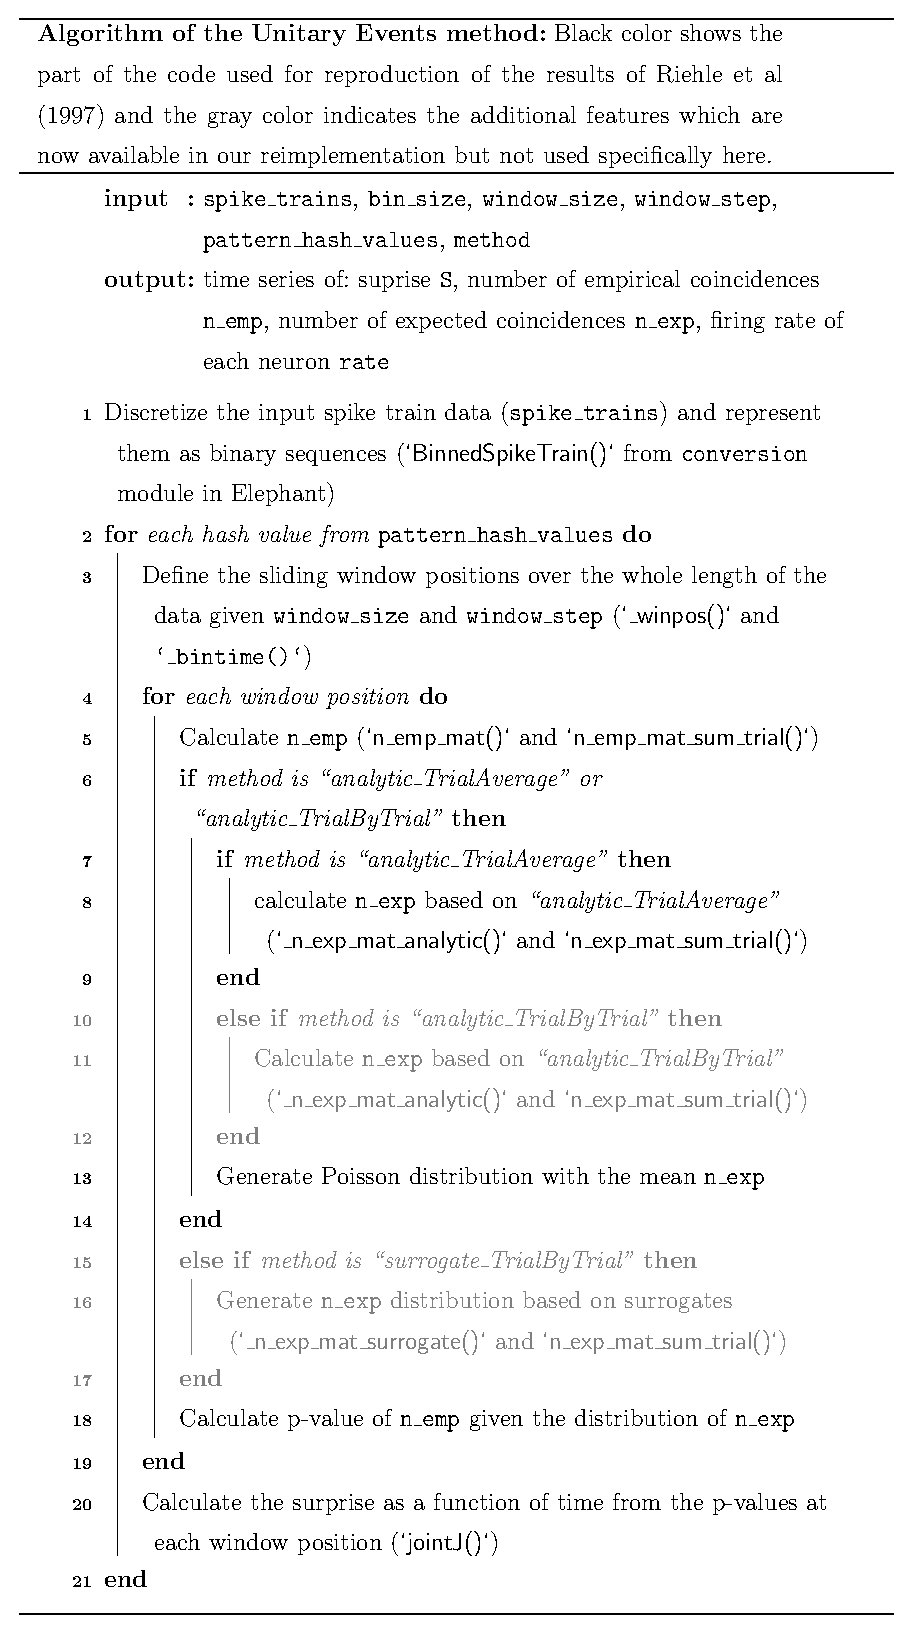
\includegraphics{UE_algorithm.eps}\\
cross-trial variability, the \emph{``analytic\_TrialByTrial''} method
(line 10 in the pseudo code) should be used, which accounts for
cross-trial changes in the firing rates by computing the expected number
of occurrences of the spike pattern based on the product of single-trial
estimates of firing rates \autocite{Gruen03b}. Both methods perform a
parametric test, where the number of occurrences of the spike pattern is
assumed to be a Poisson-distributed. As an alternative non-parametric
option, selecting \emph{``surrogate\_TrialByTrial''} as
\emph{\texttt{method}} (line 15 in the pseudo code) will numerically
compute the distribution of the expected number by implementing the
null-hypothesis based on surrogate spike trains \autocite{Gruen09}. In
the following, we will explain these methods in greater detail.

In case of selecting \emph{``analytic\_TrialAverage''} - as used in the
remainder of this study for the reproduction of \autocite{Riehle97} -
the number of spikes per neuron within the sliding window is summed
across trials and divided by the number of trials and bins contained,
thus yielding the average probability \(p_{i}\) to have a spike of
neuron \(i\) in a bin of the time window. The probability to find a
particular pattern by chance in a bin is then computed by multiplication
of the relevant probabilities, e.g.~for a pattern {[}1,0,1{]} the
probability \(p\) of occurrence is given by
\(p_{[1,0,1]}=p_{1}*(1-p_{2})*p_{3}\). Note that (\(1-p_{2}\)) is the
probability for neuron 2 to contribute no spike to the pattern. The
expected number of pattern occurrences, computed as the product of the
occurrence probability \(p\) of the pattern, e.g. \(p_{[1,0,1]}\), and
the number of bins (across all trials) covered by the sliding window.
The distribution of pattern occurrence numbers is given by a Poisson
distribution with the mean equal to the expected number.

Alternatively, for the \emph{``analytic\_TrialByTrial''} method, the
firing probability of each neuron is calculated in a trial-by-trial
manner based on the spike counts per trial. The probability \(p\) of
finding the pattern by chance is calculated by summing the products of
the firing probabilities obtained individually from each trial. As for
the trial-averaging method, the expected number of pattern occurrences
is given by multiplication with the number of bins of the trial in the
sliding window, used as the mean of a Poisson distribution to obtain the
distribution of expected pattern occurrence numbers.

As a third alternative, a surrogate method for estimating the expected
number can be selected using \emph{``surrogate\_TrialByTrial''} for the
parameter \emph{\texttt{method}}. In this Monte-Carlo approach, a
surrogate version of the spike trains is generated repeatedly, and from
each surrogate the number of occurrences of the pattern of interest is
counted. The method by which surrogates are generated from the input
spike trains is spike time randomization of the spikes per trial and per
neuron within the sliding window. The pattern counts obtained from this
procedure form a distribution of the expected number of occurrences of
the pattern, thus implementing the null-hypothesis under the constraints
implied by the surrogate method.

The distribution obtained by either of the three methods above is then
used for the significance test of the pattern on the basis of the
empirical occurrence count. The p-value resulting from the test is then
transformed by a logarithmic transformation to the surprise value (line
20 in the pseudo code), which indicates by positive or negative values
more or less occurrences of the pattern than expected by chance,
respectively. If the p-value is below a fixed prescribed level
(e.g.~below \(5\%\), which corresponds to a surprise value exceeding
\(1.27\)), the occurrences of the spike pattern under investigation in
the sliding window are marked as UEs for that pattern. This procedure is
performed for each pattern of interest, and in each sliding window.

In the present study, in order to reproduce the original results we used
the \emph{``analytic\_TrialAverage''} method, which reflects the
analysis performed in the original publication \autocite{Riehle97}. The
\emph{``analytic\_TrialByTrial''} and \emph{``surrogate\_TrialByTrial''}
methods are extensions of the original UE method, which were developed
after the original publication and introduced in subsequent works
\autocites{Gruen03b}{Gruen09}.

Our reimplementation of the UE method is based on the data object model
provided by the Neo library, upon which the Elephant library is based.
The Neo library provides loading routines for a variety of data formats,
including proprietary and generic data formats. The data sets available
for reproducing Figures 2 and 4A of \autocite{Riehle97} were
tab-separated ASCII text files containing two columns of integers
(informally often referred to as ``GDF-format''): the first column
provides event codes (behavioral events or neuron IDs), and the second
column contains the time of the occurrence of these events (time
stamps). The units of the time stamps are not contained in the data
file. We partly extracted metadata information, in particular the time
units and the meaning of the event codes, from a Matlab routine
(provided by AR) operating on the GDF data file. However, only after
further communication with AR we were able to identify the exact meaning
of the content of the data files. Using this information, we wrote a new
loading routine that loads the GDF data as Neo data objects.

Our reimplementation uses the \texttt{conversion} module of Elephant for
converting the spike data (represented as a series of timestamps) into
the binary sequence to guarantee a unique, global binning mechanism for
all analysis methods provided in Elephant. The bin size to be set for
the analysis was extracted from the original publication. However,
defining the time point to start the binning of each single trial data
required to know the alignment event in each trial and how much time
before this event (pre-time) is considered. Since this information was
not documented in the original paper, we tried several possibilities
until we got an agreement with the original figures as will be shown in
the Results.

To check if our Python implementation produces the same results as the
implementation(s) used in the original publication, we compare each of
our figures in detail with the original figures. For this comparison, as
the original results used to generate these figures are not available to
us, we first extract the times of the spikes and unitary events from the
vector graphic image (PDF) in the original paper. Then, we directly
compare these times to the times of spikes and unitary events in our
reproduced results by plotting the former against the latter, as well as
examining the distribution of the differences between them.

\section{Results}\label{results}

For the reproduction of the original results in \autocite{Riehle97}, we
have to focus on reproducing Figure 2A-F and Figure 4A, since for the
rest of the figures data were either incomplete in respect to metadata
(original Figure 3) or not available (original Figure 4B,C). Figure 2
represents the main result of the study and includes the UE analysis
that underlies the subsequent analyses. Figure 4A is an example of the
application of the UE method to data with more than 2 neurons. In terms
of complexity of the code the implementation of the UE analysis for
three or more neurons is considerably more demanding than for only two
neurons. With this example we show that our implementation is capable of
performing the UE analysis for the generic case of arbitrary number of
neurons.

We apply our reimplementation of the UE method to preprocessed versions
of the spike train data available to us after communication with AR,
which in part were identical to those used in the original analysis.
Also, we learned from AR that Figure 2 was generated by the Matlab
implementation of the UE method while all remaining figures of the
original publication, including Figure 4A, were generated by the older
implementation in IDL (see Methods regarding versions of the original
code).

\begin{figure}[htbp]
\centering
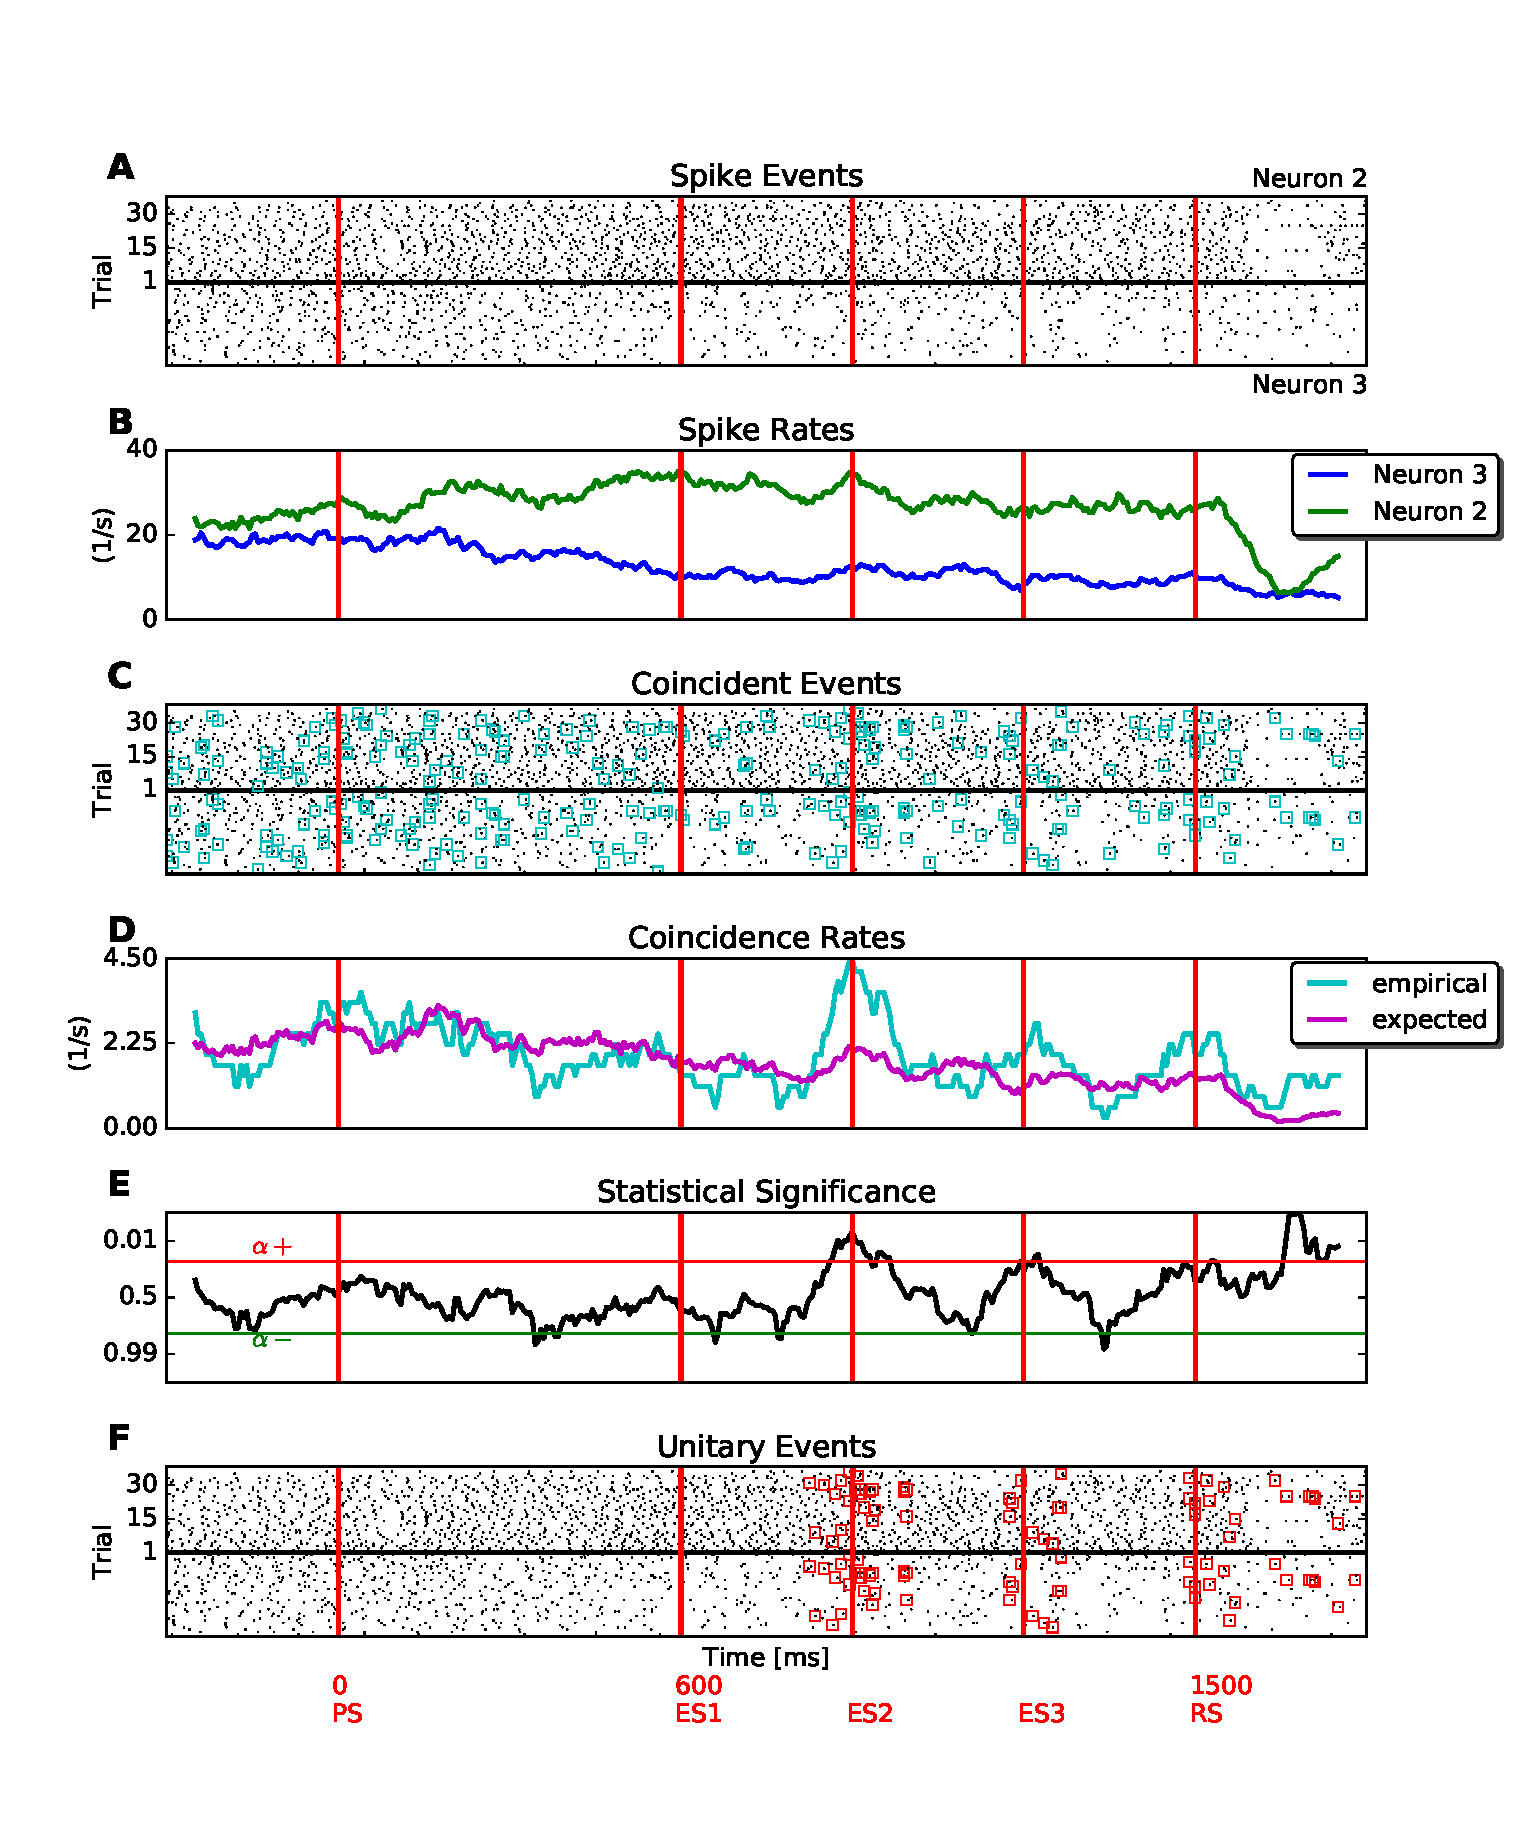
\includegraphics{figure1.eps}
\caption{\label{fig:figure2alignedPS}Initial attempt to reproduce Figure
2 of the original publication with trial alignment to PS. \textbf{A)}
Raster plot of two neurons (neuron 2: top of panel; neuron 3: bottom of
panel) in 32 trials (sorted identically for both neurons). \textbf{B)}
Average firing rate of each neuron calculated across trials in a sliding
window of length 100 ms in steps of 5 ms. \textbf{C)} Same raster plot
as in panel A with spike coincidences (i.e., pattern {[}1,1{]}) between
the two neurons marked by cyan squares. \textbf{D)} Empirical (cyan) and
expected (magenta) number of coincidences calculated in a time-resolved
manner (parameters of sliding window identical to panel B). \textbf{E)}
Time course of the surprise measure, calculated in same sliding windows
as in panel B. Surprise values that correspond to positive and negative
significance levels \(\alpha+=0.05\) and \(\alpha-=0.95\) are shown with
by horizontal red and green lines, respectively. \textbf{F)} Same raster
plot as in panel A with significant coincidences, i.e.~UEs, marked by
red squares.}\label{fig:figure2alignedPS}
\end{figure}

\begin{figure}[htbp]
\centering
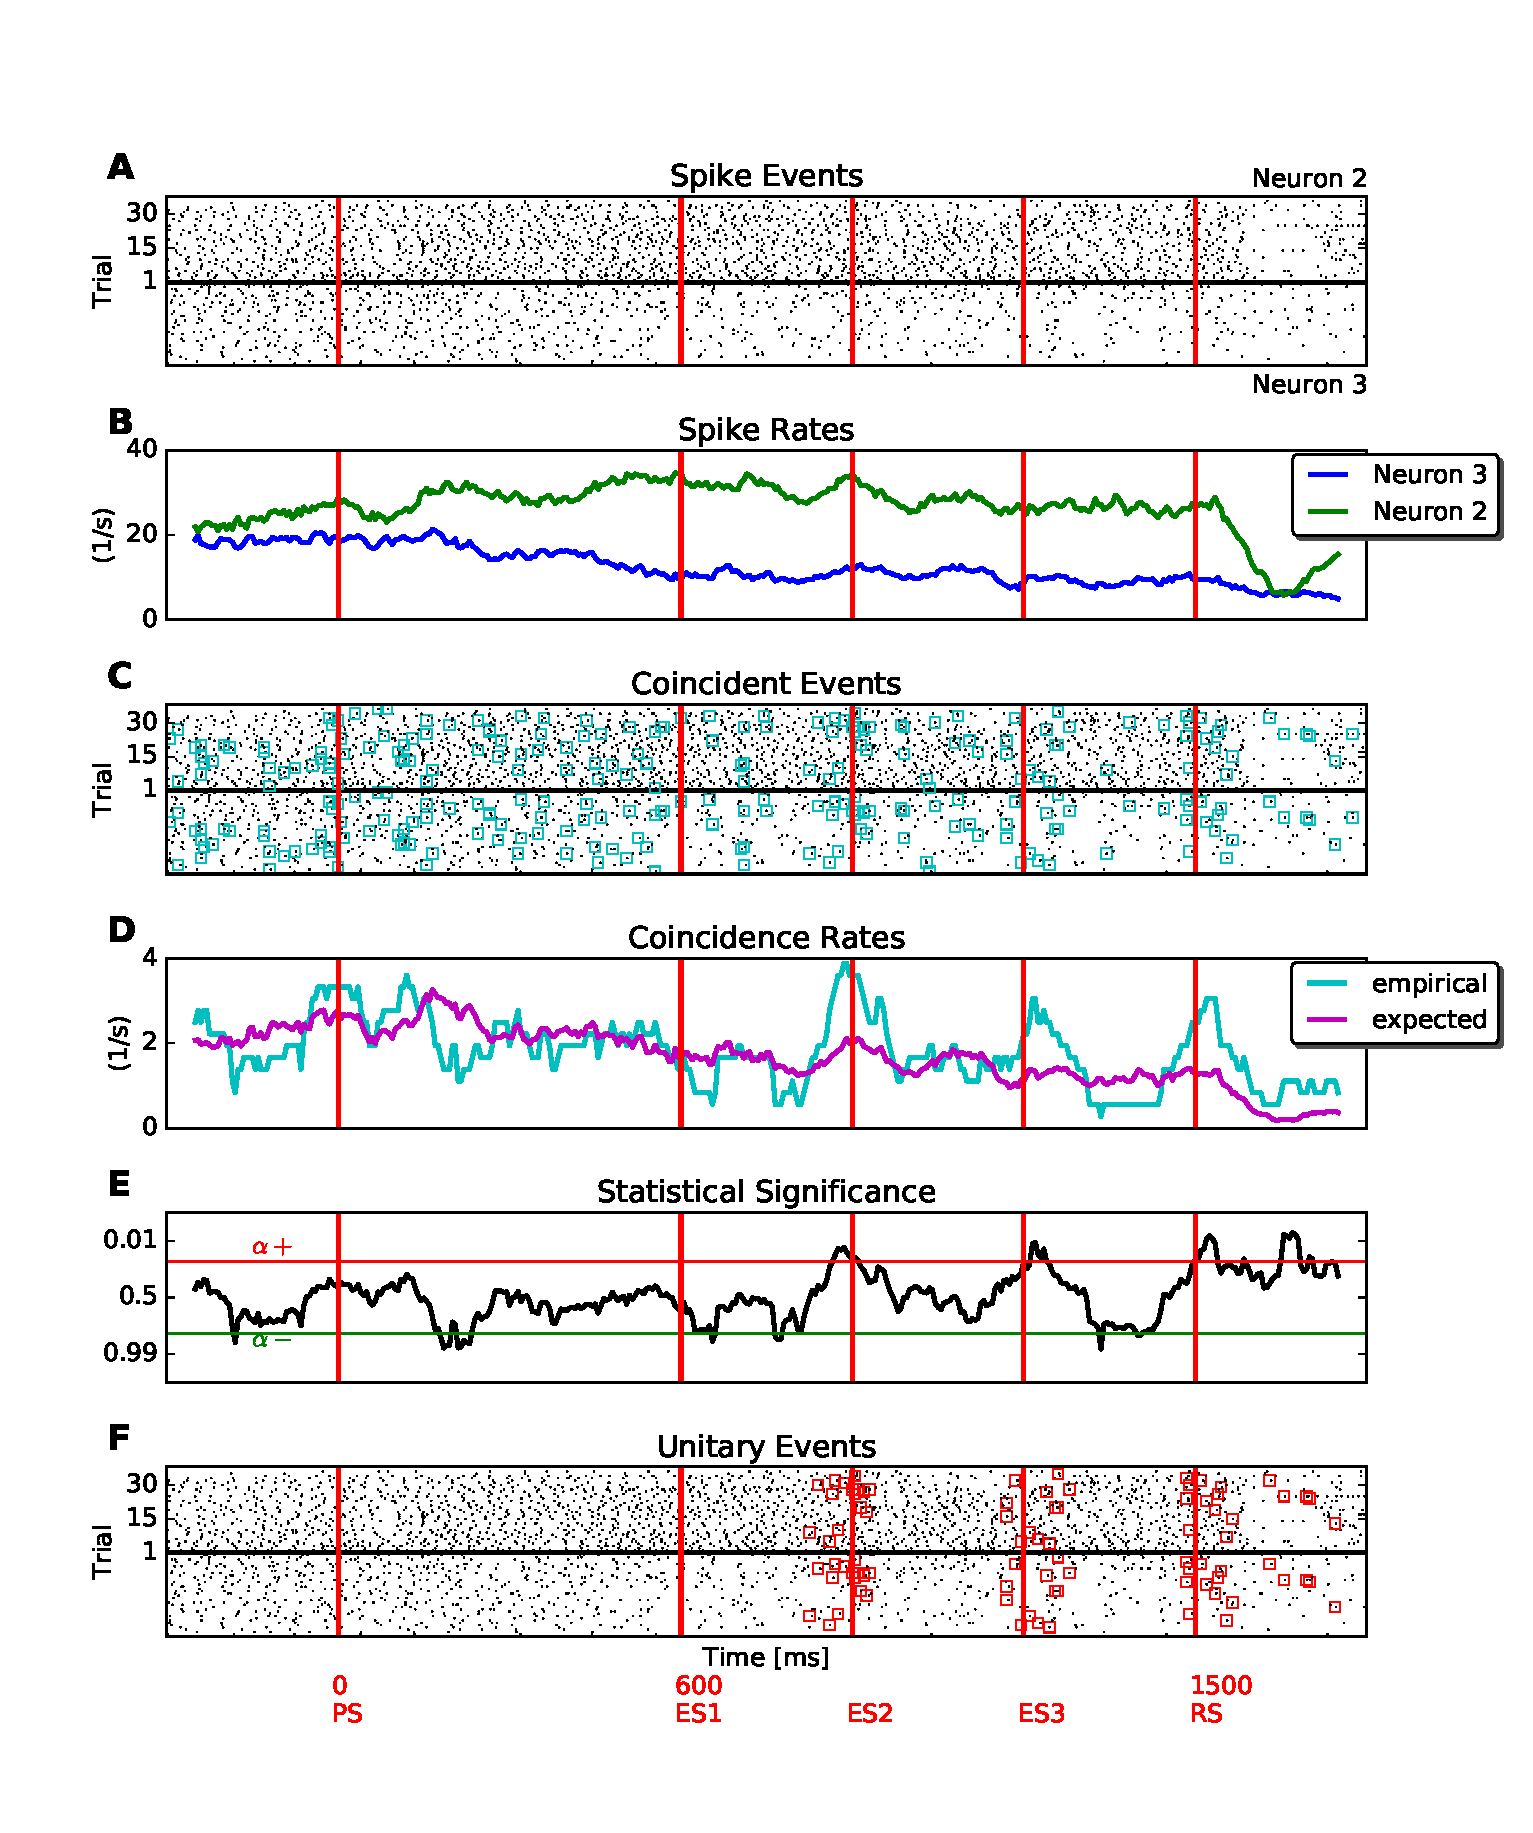
\includegraphics{figure2.eps}
\caption{\label{fig:figure2alignedRS}Reproduction of Figure 2 of the
original publication with trial alignment to RS. The same conventions as
in Figure ~\ref{fig:figure2alignedPS} apply to the respective
panels.}\label{fig:figure2alignedRS}
\end{figure}

Let us start with the reproduction of Figure 2 of the original
publication. We first give a brief description of the experiment (see
the original publication for details). After the monkey was presented
with the preparatory signal (PS) he had to sit still and wait for a
response signal (RS) to start his arm movement (i.e.~equivalent to a GO
signal). The duration of the waiting period was randomly selected on a
trial-by-trial basis to be either 600, 900, 1200 or 1500 ms. In Figure 2
of \autocite{Riehle97} only trials of the longest waiting period (1500
ms) were used for the analysis. In these trials, times marked as
expected signals ES1, ES2, and ES3 corresponded to the ends of the three
shorter waiting periods, at which the monkey could have gotten the RS
signal but did not. As the monkey was trained to recognize and
distinguish the four waiting periods, but was not informed of the
randomly selected period for a given trial, ES1-ES3 were time points at
which the monkey expected that a signal could occur.

Since the data file for Figure 2 contained the data as a continuous
recording of one recording session (``winny131.gdf''; 2 neurons, and
behavioral events), we extract the trials by cutting the data in a time
window around specific trigger events that belong to trials of the
longest waiting period, such that the complete trial is contained in the
cut-out. In a subsequent step, the spike times in the individual trials
are aligned to the trigger event, such that spike times in each trial
are given as relative to the trigger.

The original publication does not provide information which event was
used as the trigger. In this experiment, 2 events that occur in every
trial could serve as trigger events, the preparatory signal PS (event
code 114) and the response signal RS (event code 124). We noticed that
the time interval between PS and RS for the longest trials was not
identical across the respective trials and varied by \(\pm\) 1 ms. Given
the UE method is applied on a time scale of 5 ms, the analysis results
therefore are expected to depend on whether trials are aligned to PS or
RS. Thus, we decide to generate the results for both alignments.

Figures~\ref{fig:figure2alignedPS} and ~\ref{fig:figure2alignedRS} show
the results of performing the UE analysis for PS- and RS-aligned data,
respectively. Here, the analysis parameters are set to the identical
values as reported in the original publication (bin size: 5 ms, analysis
time window size: 100 ms, time step of the sliding window: 5 ms,
significance level \(\alpha= 0.05\)). The comparison of the two figures
to the original figure shows agreement in the raster displays (panel A)
and the time-resolved, trial-averaged firing rate estimates (B).
However, although the graphs of the number of coincidences per sliding
window (panel D) and the surprise measure (panel E) are similar in their
overall general behavior, they differ in the details. Thus, indeed the
choice of the alignment influences the analysis result. In order to test
if one of the two alignments is in agreement with the original
publication, we perform a detailed visual comparison of our two figures
and the original one on the basis of the spikes marked as coincident
(panels C) and as part of a UE (panel D). We notice that when aligning
to PS (Figure~\ref{fig:figure2alignedPS}), the marked spikes do not
agree in all details with the original figure. However, in
Figure~\ref{fig:figure2alignedRS}, with trials aligned to RS, we find no
disagreements with the original figure. After this visual comparison we
check if our results are exactly identical to the original ones.
Therefore, we extract the positions of the data points representing
spikes and UEs in the original figure by reading the plotting commands
in the PDF file of the original paper, and compare them to our
reproduced results. In Figure~\ref{fig:validation_fig2} A the reproduced
spike times in Figure~\ref{fig:figure2alignedRS} A are plotted against
the extracted original spike times. The plotted data points lie on the
diagonal line, indicating that the reproduced spike times correspond to
the original ones. Figure~\ref{fig:validation_fig2} B shows the same
plot for the UEs, indicating the identity of the original and reproduced
UE timings as well. To further confirm the identity, we plot the
distributions of the differences between the original and the reproduced
timings for the spikes (Figure~\ref{fig:validation_fig2} C; black) and
the UEs (Figure~\ref{fig:validation_fig2} D). The differences are at
most +/- 0.3 ms, which are considerably narrower than the +/- 1 ms
differences caused by the misaligned data shown in
Figure~\ref{fig:figure2alignedPS} A (see for comparison the gray plot in
Figure~\ref{fig:validation_fig2} C, which shows the differences between
the original spike times and the misaligned spike times). The remaining
minor differences of the spike and UE times of the correctly aligned
data and the original data are only due to slight errors in the
extraction of the spike times from the original figure, which is
inevitable because of a limited precision of the plotting commands in
the PDF file. Thus, we confirm that spike timings in the correctly
aligned data are identical to those in the original data, and our
implementation of the UE analysis applied to these data reproduces
exactly the same results as shown in the original paper.

\begin{figure}[htbp]
\centering
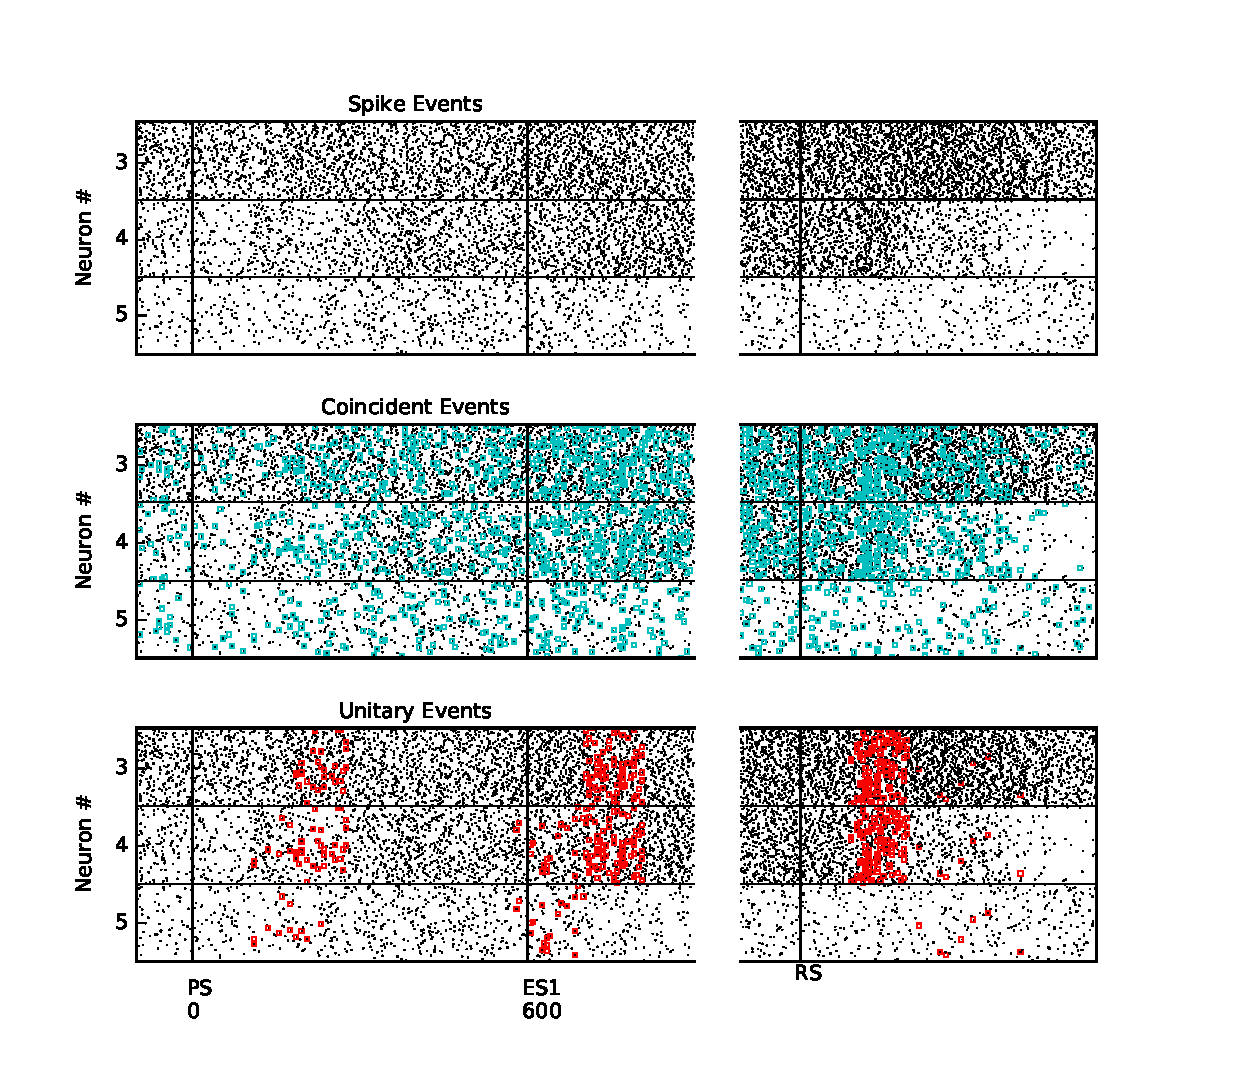
\includegraphics{figure3.eps}
\caption{\label{fig:validation_fig2}\textbf{A)} The scatter plot of the
reproduced spike times in Figure~\ref{fig:figure2alignedRS} A plotted
against the extracted original spike times. \textbf{B)} Same plot as in
A but for the time of occurrences of UEs. \textbf{C)} The distributions
of the differences between the original and the reproduced timings for
spikes in Figure ~\ref{fig:figure2alignedRS} and
Figure~\ref{fig:figure2alignedPS} are shown in black and gray,
respectively. \textbf{D)} Same plot as in C but for UEs in Figure
~\ref{fig:figure2alignedRS}.}\label{fig:validationux5ffig2}
\end{figure}

As a next step we aim at reproducing Figure 4A of \autocite{Riehle97}.
This figure contains the result of the analysis of three neurons
recorded simultaneously, in contrast to Figure 2 where only two neurons
are considered. We analyze the original data for this figure provided by
AR with the parameter values given in \autocite{Riehle97} and compare
our result to the original figure. Figure 4A of the original publication
contains the raster displays of the data in the top panel, the raster
displays with the marked coincident spikes (blue marks) in the middle
panel, and the raster displays with the marked spikes that are part of a
UE (red marks) in the bottom panel. We find that the UE result is
different, as the UEs occur at different times and between different
neurons compared to the original publication. Thus we check whether the
spike times of the individual spikes are identical between the original
and our results. Figure~\ref{fig:comparison_raster} shows a segment of
the raster plot of the original figure and the corresponding segment of
our reproduced figure. We compare the positions of the single spikes and
find that there are small discrepancies between the two raster plots in
some of the spike times. Figure~\ref{fig:comparison_raster} shows
examples of clusters of spikes marked in red that should be identical in
both raster plots but contain a few individual spikes that are slightly
shifted in our figure compared to the original figure by a very small
amount.

\begin{figure}[htbp]
\centering
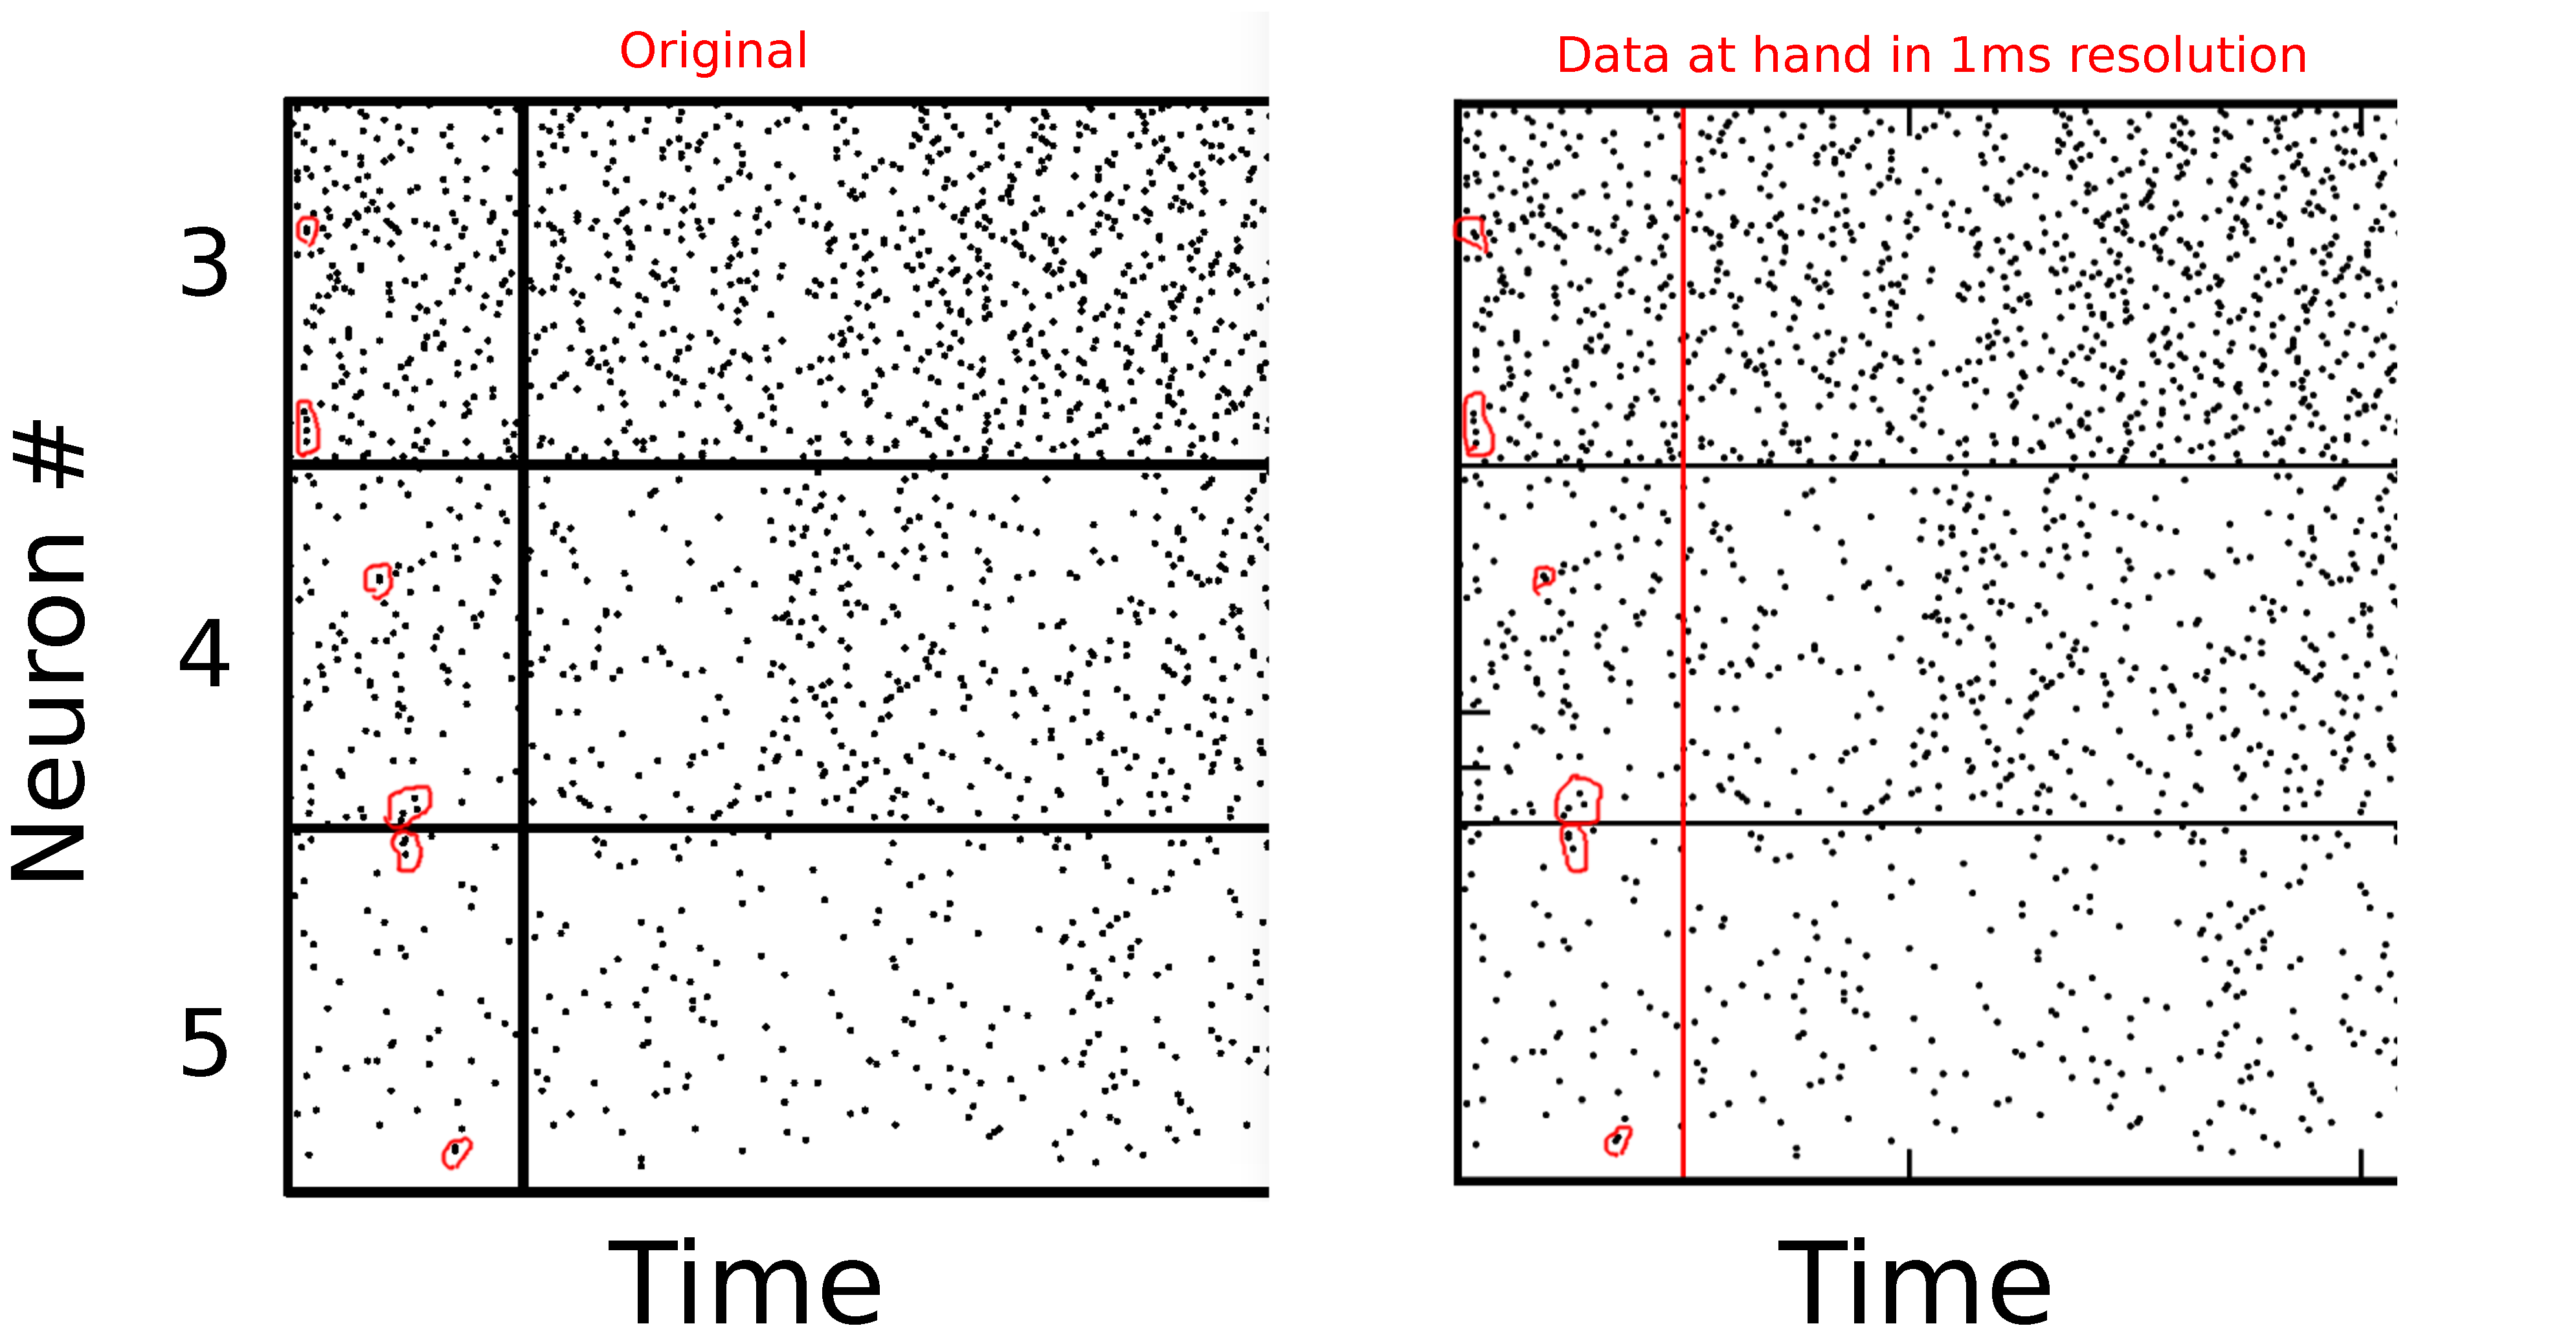
\includegraphics{PS_aligned_matlabdata_marked.eps}
\caption{\label{fig:comparison_raster}Close-ups of the original raster
display in Figure 4A of the original publication (left) and the first
data file available at hand for reproduction (right) reveal slight
differences in the positions of some spikes. Data on the right are
aligned (similar to the data on the left) to ES1 (event code 15 in the
GDF data file). The time before the alignment event is chosen as 700 ms,
and a bin size of 5 ms is used. The red marks indicate spike clusters
with identified differences between the left and the right panel, where
at least one spike is shifted in the right panel compared to the left
one.}\label{fig:comparisonux5fraster}
\end{figure}

This leads us to the suspicion that the data are binned in a fashion
that is not consistent with the data shown in the original publication.
Personal communication with AR revealed that while Figure 2 had been
generated by the Matlab implementation of the UE analysis, Figure 4 had
been generated by the IDL implementation (see Introduction). A report by
MD written before the time of the original publication summarized a
comparison of the IDL and the Matlab implementations, and concluded that
both were correct implementations of the method, but differed in their
results due to a slightly different implementation of the down-sampling
and binning of the raw data (recorded at 10 kHz). In the workflow for
the IDL implementation, as illustrated in
Figure~\ref{fig:workflow_report} (the leftmost branch of the diagram),
the raw data were first down-sampled to a temporal resolution of 0.5 ms
(by a program \texttt{2gdf}) and then further rounded to 1 ms resolution
integer values inside the IDL implementation. The data available to us
had a resolution of 1 ms, which must have been a result of another
down-sampling procedure than the one for the IDL implementation. This
explains the difference in the raster displays, and this difference is
likely also the cause that we were initially not able to reproduce the
original UE result.

\begin{figure}[htbp]
\centering
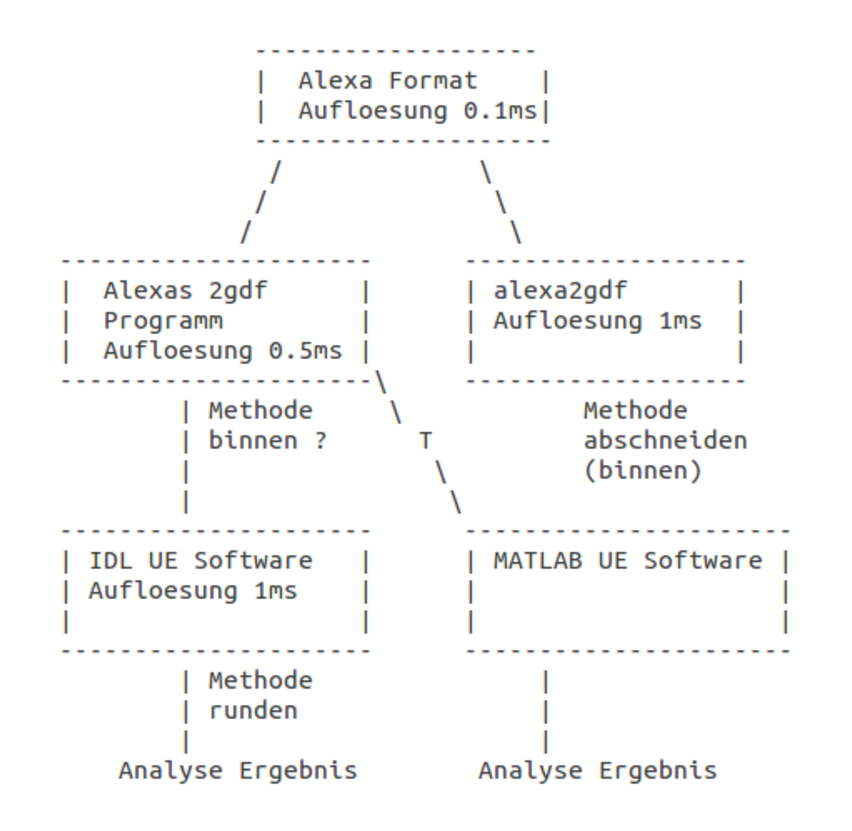
\includegraphics{CmpIDL_Matlab_3.eps}
\caption{\label{fig:workflow_report}Illustration of the data
preprocessing workflow, translated from the 1997 report of MD (in
German) on the comparison of the first UE implementation in IDL (left
branch) and the second implementation in Matlab
\autocite{Diesmann16_personalcomm} (right branch). Data entering both
analysis branches have a resolution of 0.1 ms (top box). In the IDL
branch spike times \(t\) in the original data are first transformed to a
resolution of \(h=0.5\) ms (by the \texttt{2gdf} program, middle left)
using the method of binning \(\lfloor t/h \rfloor\). Then the data are
read into the ``IDL UE Software'' (lower left box) and therein converted
to \(h=1\) ms resolution by the method of ``round half up''
\(\lfloor t/h+1./2 \rfloor\) prior to analysis. Alternatively, one can
load the 0.5 ms resolution data into the ``MATLAB UE Software'' (lower
right box). Here the bin width is a parameter of the analysis and thus
data can be converted to a 1 ms resolution but results are different
from the IDL branch. Results are only identical if a prior
transformation ``T'' (diagonal in center) performs a round half up and
no further binning is done in the MATLAB program. At a later point in
time the \texttt{alexa2gdf} converter function (written in MATLAB)
became available such that data in the original 0.1 ms resolution could
directly be converted to the 1 ms resolution by binning. The full report
(``Report\_by\_MarkusDiesmann.txt'') is included in the data folder of
the repository for this paper.}\label{fig:workflowux5freport}
\end{figure}

In our reproduction of Figure 2 of the original paper we use
preprocessed data available in 1 ms resolution, that likely experienced
the \texttt{alexa2gdf} program for conversion as shown in
Figure~\ref{fig:workflow_report} (the rightmost branch), before data are
loaded into our reimplementation of the UE analysis. However, according
to the aforementioned report by MD, we only have a chance to reproduce
Figure 4A of \autocite{Riehle97} if we have the original data or a
version of them with a time resolution lower than 1 ms available. The
original raw data with 0.1 ms resolution are presumably only available
on a storage medium and format that at present we are not able to read
and interpret. However, after we contacted AR she found the data
(``jenny201\_345\_preprocessed.gdf'') of Figure 4A of
\autocite{Riehle97} with a time resolution of 0.5 ms, which likely
experienced the \texttt{2gdf} program for conversion (middle left box in
Figure~\ref{fig:workflow_report}).

We loaded this data at 0.5 ms resolution into Python and converted the
data from the 0.5 ms to the required 1 ms resolution by the mathematical
operation \(\left\lfloor x+\frac{1}{2}\right\rfloor\) , called
``rounding half up''. In numerical software packages, including IDL,
this operation is typically implemented by a function named round().
However, the round() implementation of NumPy (version 1.11.0) performs
an even rounding, i.e., values exactly halfway between two integers are
rounded to the nearest even integer. Indeed, the latter implementation
of rounding did not reproduce the result of the original publication.
Thus, we used the expression \texttt{floor(x+0.5)} to perform rounding
as it is implemented by IDL. The procedure completely reproduces panel A
of Figure 4 in the original publication (see
Figure~\ref{fig:reproducedFig4A}).

\begin{figure}[htbp]
\centering
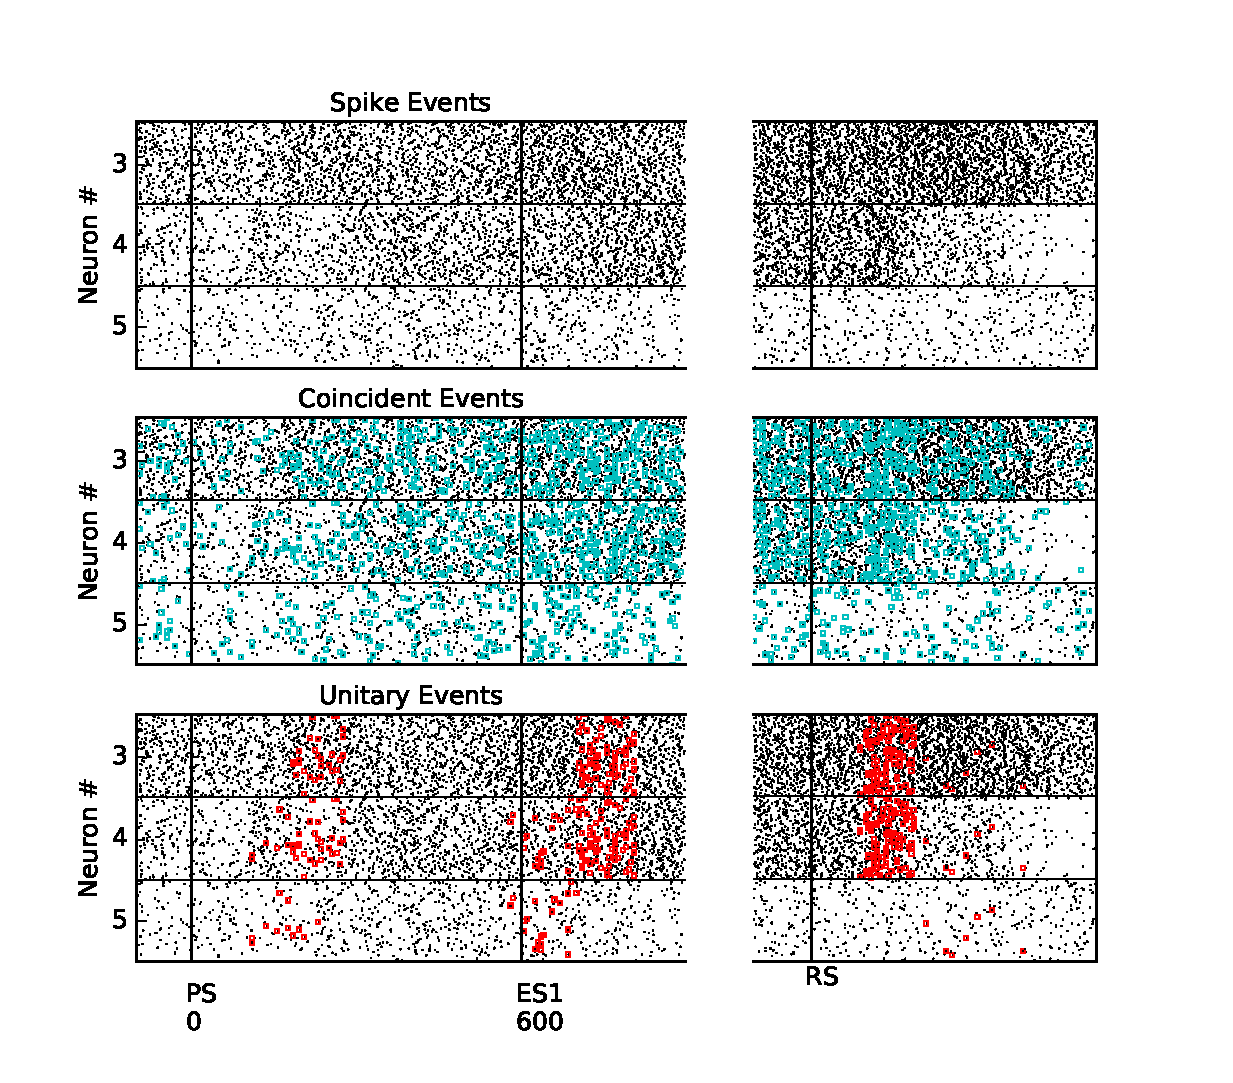
\includegraphics{figure6.eps}
\caption{\label{fig:reproducedFig4A}Reproduction of Figure 4A of the
original publication. The left part of the figure shows the UE analysis
result for the data aligned to ES1 (event code 15 in the GDF data file)
with a time before the event (pre-time) set to 699 ms. The right part of
the figure shows the analysis of the same data aligned to RS and with a
pre-time of 99 ms. The left and right parts of the figure show 96 and
128 trials, respectively.}\label{fig:reproducedFig4A}
\end{figure}

\section{Conclusion}\label{conclusion}

We are able to reproduce the original results of \autocite{Riehle97} by
applying a new reimplementation of the Unitary Events analysis method in
Python to the original data. The method involves a number of numerical
computations and is very sensitive, as we show here by the comparison of
Figures ~\ref{fig:figure2alignedPS} and ~\ref{fig:figure2alignedRS},
which differed in the events that the trials were aligned to. This
difference in the alignment would not affect the results if the time
difference between the two events (PS and RS) were identical across the
trials. But since the latter was not the case due to hardware features
of the recording setup (as we learned from the first author of the
original publication), the binning of the data started at a slightly
different time points in different trials. This likely led to a loss or
an addition of a spike in a bin and thus to a small difference of the
number of spike synchrony events (see also the discussion on the issues
of exclusive binning in \autocite{Gruen99}). In spite of this
sensitivity of the method, we succeeded in generating results that are
exactly identical to the original ones, as confirmed by the direct
comparison of the positions of spikes and UEs in the original and the
reproduced figures. This is a strong indication that our new
implementation of the analysis faithfully implemented the UE method.

The event to which the data were aligned and the cut time which then
defined the start of the (exclusive) binning was not documented in the
original publication. Also the original scripts for the analysis are not
available anymore, which could have revealed this information, even
without having the original UE software code at hand. Thus, due to the
lack of documentation we are only able to reproduce the results of
\autocite{Riehle97} by communicating with some of the authors of the
original publication.

The reproduction of Figure 4A of the original publication is a further
and important test whether our reimplementation is also correct for
N\textgreater{}2 neurons. This is relevant since the implementation
requires a more generic, complex algorithm for the analysis than the one
that can be used for only N=2. In the case of two neurons, there is only
one pattern type which has to be analyzed (i.e. {[}1,1{]}). However, in
the case of e.g.~3 neurons there are already 4 different spike patterns
to analyze ({[}1,1,0{]}, {[}0,1,1{]}, {[}1,0,1{]}, and {[}1,1,1{]}), and
even much more for more neurons (\(2^{N}-N-1\)). The statistics of each
of the patterns is performed separately and, therefore, the bookkeeping
needs to be carefully done.

The reproduction of Figure 4A is more complicated than reproducing
Figure 2 due to additional reasons. First of all, the data were not
available to us. After requesting them from the first author of the
original publication we received data and were not able to reproduce the
result - in terms of the UE results, but also the data seemed slightly
different. After further consultation with the original authors we
learned that the original Figure 4A was not generated by the Matlab
implementation used for Figure 2 but by another implementation in IDL.
Both are not available to us. However, we were told that the third
author, MD, of the original publication performed a thorough comparison
of the two implementations at the time and the final report on that
investigation was made available to us. This enables us to define the
correct workflow that reproduces the original result, given we have the
data in the correct resolution at hand.

The reimplemented UE analysis software contains extensions for improving
the statistics that were developed after the original publication. On
the one hand, it contains the option to adjust the statistics to take
into account cross-trial inhomogeneity by calculating the number of
expected spike synchrony events based on the firing rates in a
trial-by-trial fashion (option: \emph{``analytic\_TrialByTrial''}) as
suggested in \autocite{Gruen03b}, in contrast to using trial averages of
the firing rates. On the other hand, our reimplementation offers the
possibility to calculate the significance of the empirical number of
spike synchrony events based on a Monte Carlo approach (option:
\emph{``surrogate\_TrialByTrial''}). Instead of computing the
significance using a parametric distribution based on the estimate of
the firing rates, the null-hypothesis of independence is implemented by
surrogate data \autocites{Gruen09}{GruenRotter10_Chap10}{Louis10}. By
repeated intentional manipulation of the original data, potential spike
synchrony is deleted. Each of these surrogate data created by this
procedure are then searched - as the original data - for spike
synchrony, and these numbers create the distribution underlying the
significance test of the method. Obviously this version is considerably
more computationally expensive than the parametric approach used here
for the reproduction of \autocite{Riehle97} and we are currently working
on an HPC implementation to make use of parallelization. The Python
implementation of the UE method is publicly available in the open source
software package Elephant at http://neuralensemble.org/elephant/.

If the authors of the original paper would not have been accessible, we
would not have been able to reproduce the results. Nevertheless, here
our final validation of the reproduction is based on the values
extracted from the vector graphic image (PDF) in the original paper. In
an optimal scenario, we would be able to exactly validate the results
based on a numerical comparison. To do so, all of the following pieces
of information would have had to be available at hand:

\begin{enumerate}
\def\labelenumi{\arabic{enumi}.}
\item
  the original primary data
\item
  metadata describing the primary data in detail
\item
  the original statistics software package (e.g.~Unitary Events)
\item
  the loading routine for the data
\item
  all specific code required to produce each figure of the original
  publication
\item
  detailed documentation of all code
\item
  the original software environment (with programs available in the
  original versions used), including, e.g.~the interpreter/compiler
  (here: Matlab) and operating system
\item
  unique identifiers of the data records that unambiguously identify
  data from within the analysis code
\end{enumerate}

In the analysis presented in this work, not even the original primary
data (1), recorded more than 20 years ago, but only a slightly
preprocessed version is available. However, even today many of the
pieces of information listed above are often not made available by
scientists. In part, this is due to the enormous complexity of the task
to record all information in fine detail leading from the experiment to
an analysis result. Moreover, there is still a lack of software tools to
support researchers in the process of acquiring, storing, and organizing
this information. Currently, there are emerging approaches suggested for
metadata annotation (2) of electrophysiological data, such as the
odML\footnote{\url{https://github.com/G-Node/python-odml}} framework
(see, e.g. \autocites{Grewe2011}{Zehl2016}) for storing hierarchical
collections of metadata or the NIX\footnote{\url{https://github.com/G-Node/nix/wiki}}
data format \autocite{Adrian2014} for linking data and metadata. In our
concrete example, the information about the hardware limitations in
storing the event times, would have been essential information contained
in the metadata. Using modern tools for version control, points (3)-(6)
can be easily addressed. There are emerging approaches to keep software
environment, i.e., the original Matlab version and the operating system
(7), e.g., by freezing the environment in a virtual machine. Point (8)
is still challenging, because it requires the data to be addressed in an
unambiguous manner from within the analysis scripts. Including data
within the code repositories is typically prohibitive due to the size of
the data. A solution would be to deposit data in public or private
databases that allow data to be identified using a unique identifier in
combination with a tool to generate a detailed provenance track of the
analysis process, but the implementation of tools and services for the
workflows used in data analysis of electrophysiological data is still an
ongoing endeavor \autocites{badia_incf_2015}{Denker2015_000}. In
summary, there are still components missing such that researchers are
put into a position to build complex data acquisition and analysis
workflows that enable optimal reproducibility in neuroscience.

\section{Author Contribution}\label{author-contribution}

\textbf{VR}: Implementing the UE analysis in Python, Reproduction of the
figures, Discussion of the results, Drafting of the manuscript, Revision
of the draft. \textbf{JI}: Reproduction of the figures (with VR),
Discussion of the results (with all other authors), Drafting of the
manuscript (with VR), Revision of the draft (with all other authors).
\textbf{MDe}: Drafting of the manuscript (with VR), Revision of the
draft (with all other authors), Assisted in integrating the UE analysis
in the Elephant library. \textbf{SG}: Conceived the original idea of
reproduction, mediated the communications with original authors,
provided suggestions for correcting errors in intermediate reproduction
results, discussed the results, revised the manuscript (with all other
authors).

\section{Acknowledgements}\label{acknowledgements}

This project received funding from EU Grant 720270 (HBP), Deutsche
Forschungsgemeinschaft Grant DE 2175/2-1 and GR 1753/4-2 of the Priority
Program (SPP 1665), the German-Japanese Computational Neuroscience
Project (German Federal Ministry for Education and Research, BMBF Grant
01GQ1114), from the Helmholtz Portfolio Theme ``Supercomputing and
Modeling for the Human Brain'', and from the Osaka Univ for the project
`Neural mechanism of active vision studied by combining large-scale
sampling of neural activity and advanced computational analysis'.

We thank Alexa Riehle and Markus Diesmann for fruitful discussions.

{\sffamily \small
  \printbibliography[title=References]
}
\end{document}
